\documentclass{bmstu}

\usepackage{lmodern}
\usepackage[utf8]{inputenc}

\begin{document}
	
	\makereporttitle
	{Информатика, искусственный интеллект и системы управления}
	{Программное обеспечение ЭВМ и информационные технологии}
	{лабораторной работе №~1}
	{Методы вычислений}
	{}
	{9}
	{Сапожков~А.~М./ИУ7-13М}
	{Власов~П.~А.}
	
\chapter{Теоретическая часть}

\textbf{Цель работы:} изучение венгерского метода решения задачи о назначениях.

\textbf{Задание:}
\begin{enumerate}
	\item Реализовать венгерский метод решения задачи о назначениях в виде программы на ЭВМ.
	\item Провести решение задачи с матрицей стоимостей, заданной в индивидуальном варианте, рассмотрев два случая:
	\begin{itemize}
		\item задача о назначениях является задачей минимизации,
		\item задача о назначениях является задачей максимизации.
	\end{itemize}
\end{enumerate}

\section{Cодержательная и математическая постановки задачи о назначениях}

\textbf{Содержательная постановка:} имеется $n$ работ и $n$ исполнителей; стоимость выполнения $i$-ой работы $j$-ым исполнителем составляет $c_{ij} \geq 0$ единиц. Требуется распределить все работы между исполнителями так, чтобы
\begin{itemize}
	\item каждый исполнитель выполнял 1 работу;
	\item общая стоимость выполнения всех работ была $min$.
\end{itemize}

Введём управляемые переменные:
\begin{equation}
	x_{ij}  =
	\begin{cases}
		1, \text{если $i$-ую работу выполняет $j$-ый работник}, \\
		0, \text{иначе};
	\end{cases} \nonumber \\
	i, j  = \overline{1; n}. 
\end{equation}

Из переменных $x_{ij}$, $i,j = \overline{1; n}$, составим 
\begin{equation}
	X = (x_{ij})_{i,j = \overline{1; n}},
\end{equation}
которую назовём матрицей назначений.

Стоимости выполнения работ также записываем в матрицу
\begin{equation}
	C = (c_{ij})_{i,j = \overline{1; n}},
\end{equation}
называемой матрицей стоимостей.

Тогда:
\begin{enumerate}
	\item Стоимость выполнения работ:
	\begin{equation}
		f = \sum_{i=1}^n \sum_{j=1}^n c_{ij} x_{ij}.
	\end{equation}
	\item Условие того, что $i$-ую работу выполнит ровно один работник:
	\begin{equation}
		\sum_{j=1}^n x_{ij} = 1, \: i = \overline{1; n}.
	\end{equation}
	\item Условие того, что $j$-ый работник выполнит ровно одну работу:
	\begin{equation}
		\sum_{i=1}^n x_{ij} = 1, \: j = \overline{1; n}.
	\end{equation}
\end{enumerate}

Таким образом приходим к \textbf{математической постановке}:
\begin{equation}
	\begin{cases}
		f = \sum_{i=1}^n \sum_{j=1}^n c_{ij} x_{ij} \rightarrow min, \\
		\sum_{j=1}^n x_{ij} = 1, \: i = \overline{1; n}, \\
		\sum_{i=1}^n x_{ij} = 1, \: j = \overline{1; n}, \\
		x_{ij} \in \{0, 1\}, \: i,j = \overline{1; n}.
	\end{cases}
\end{equation}

\section{Исходные данные варианта №9}

\begin{equation}
	C = 
	\begin{bmatrix}
		4 & 7 & 1 & 5 & 5 \\
		6 & 8 & 3 & 7 & 6 \\
		6 & 4 & 5 & 7 & 7 \\
		4 & 2 & 3 & 4 & 9 \\
		8 & 1 & 8 & 3 & 8
	\end{bmatrix}
\end{equation}

\section{Краткое описание венгерского метода}

Схема венгерского метода решения задачи о назначениях представлена на рисунках \ref{img:1}-\ref{img:3}.

\begin{figure}[h!]
	\begin{center}
		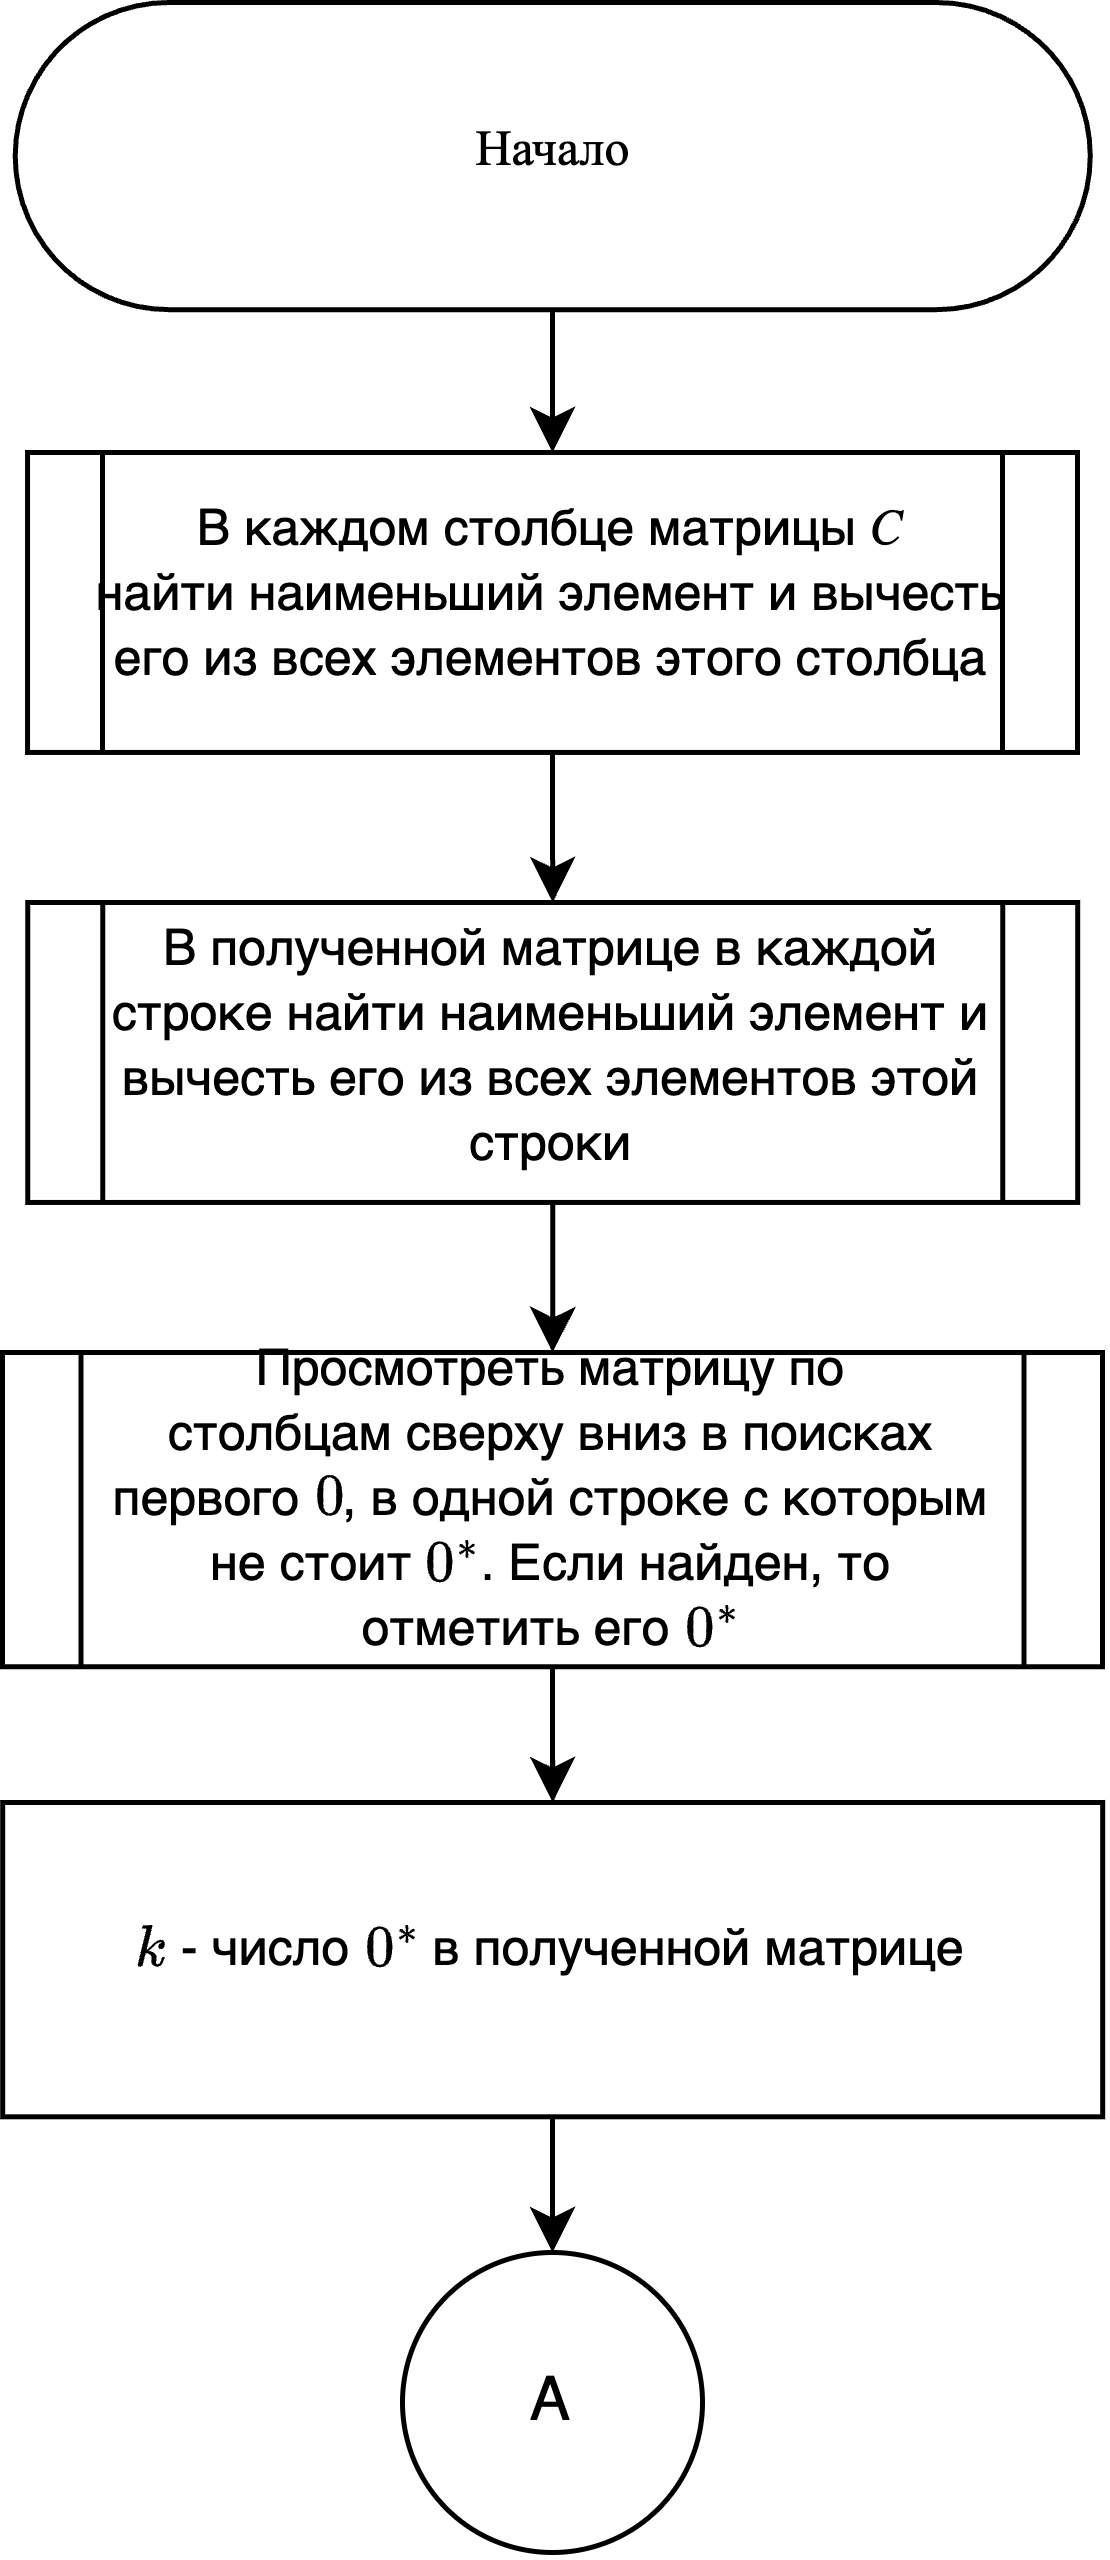
\includegraphics[scale=0.2]{inc/img/1.png}
	\end{center}
	\caption{Схема венгерского метода решения задачи о назначениях, часть 1}
	\label{img:1}
\end{figure}

\begin{figure}[h!]
	\begin{center}
		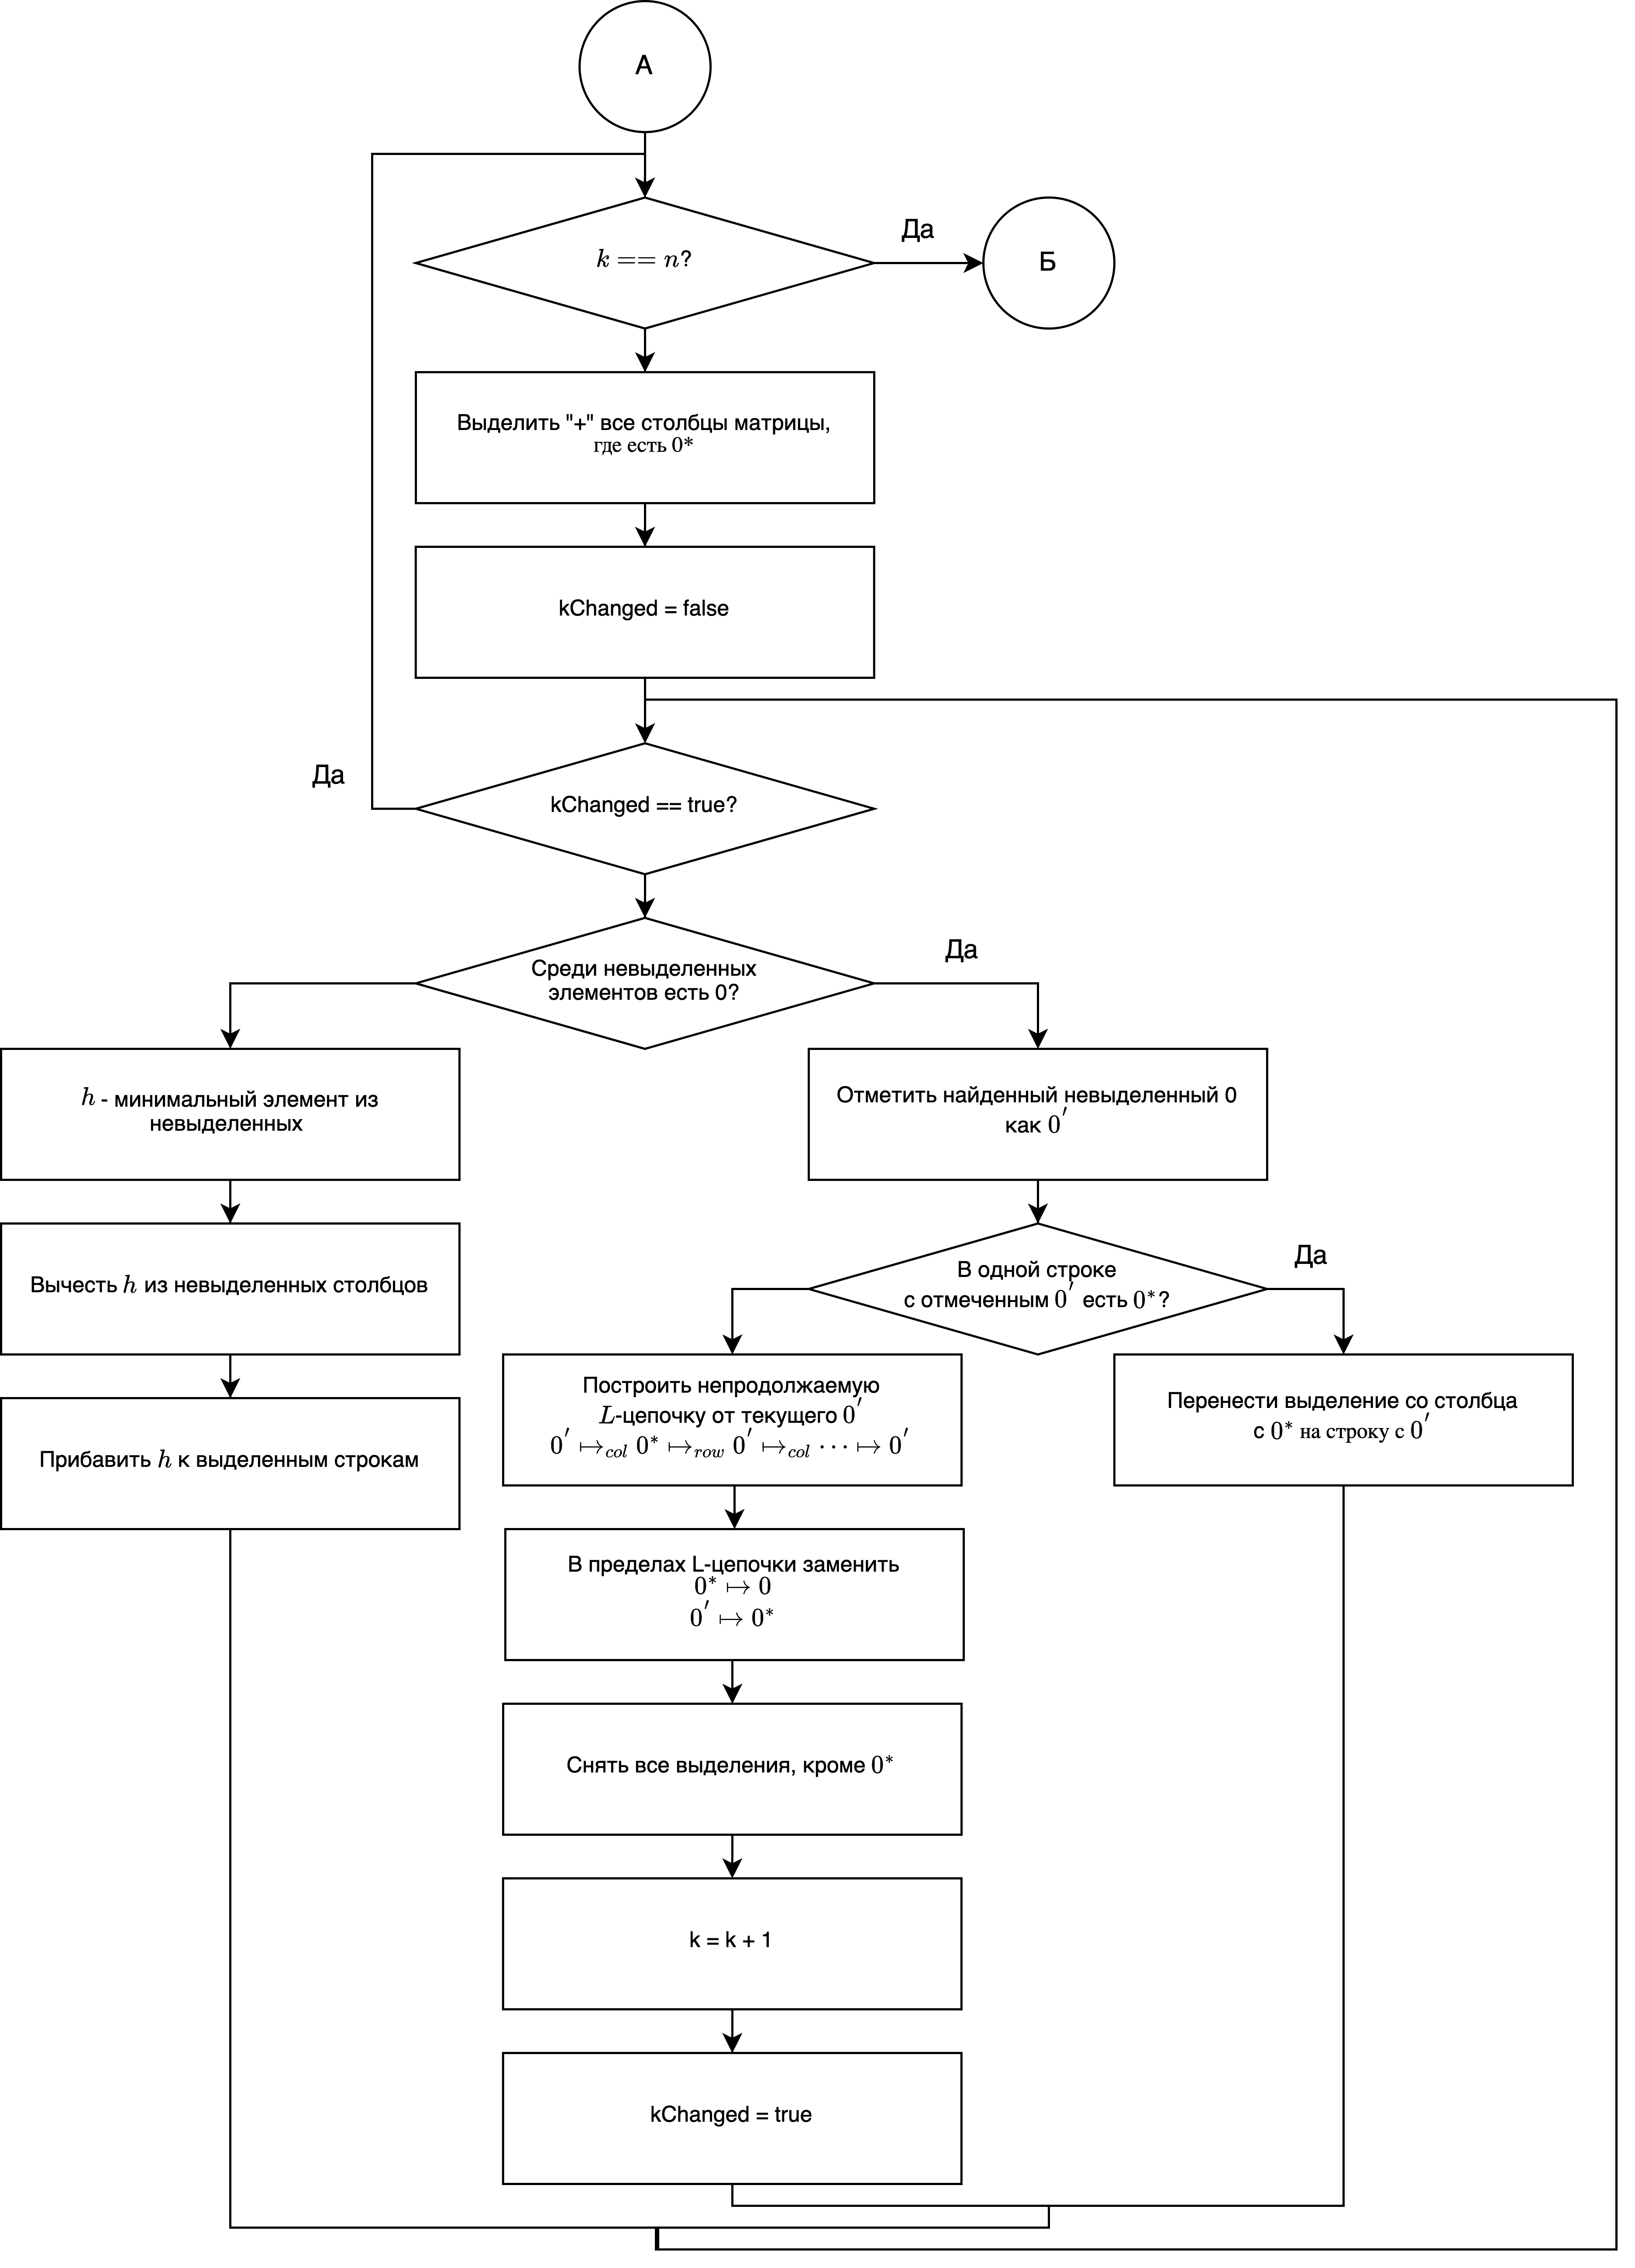
\includegraphics[scale=0.13]{inc/img/2.png}
	\end{center}
	\caption{Схема венгерского метода решения задачи о назначениях, часть 2}
	\label{img:2}
\end{figure}

\begin{figure}[h!]
	\begin{center}
		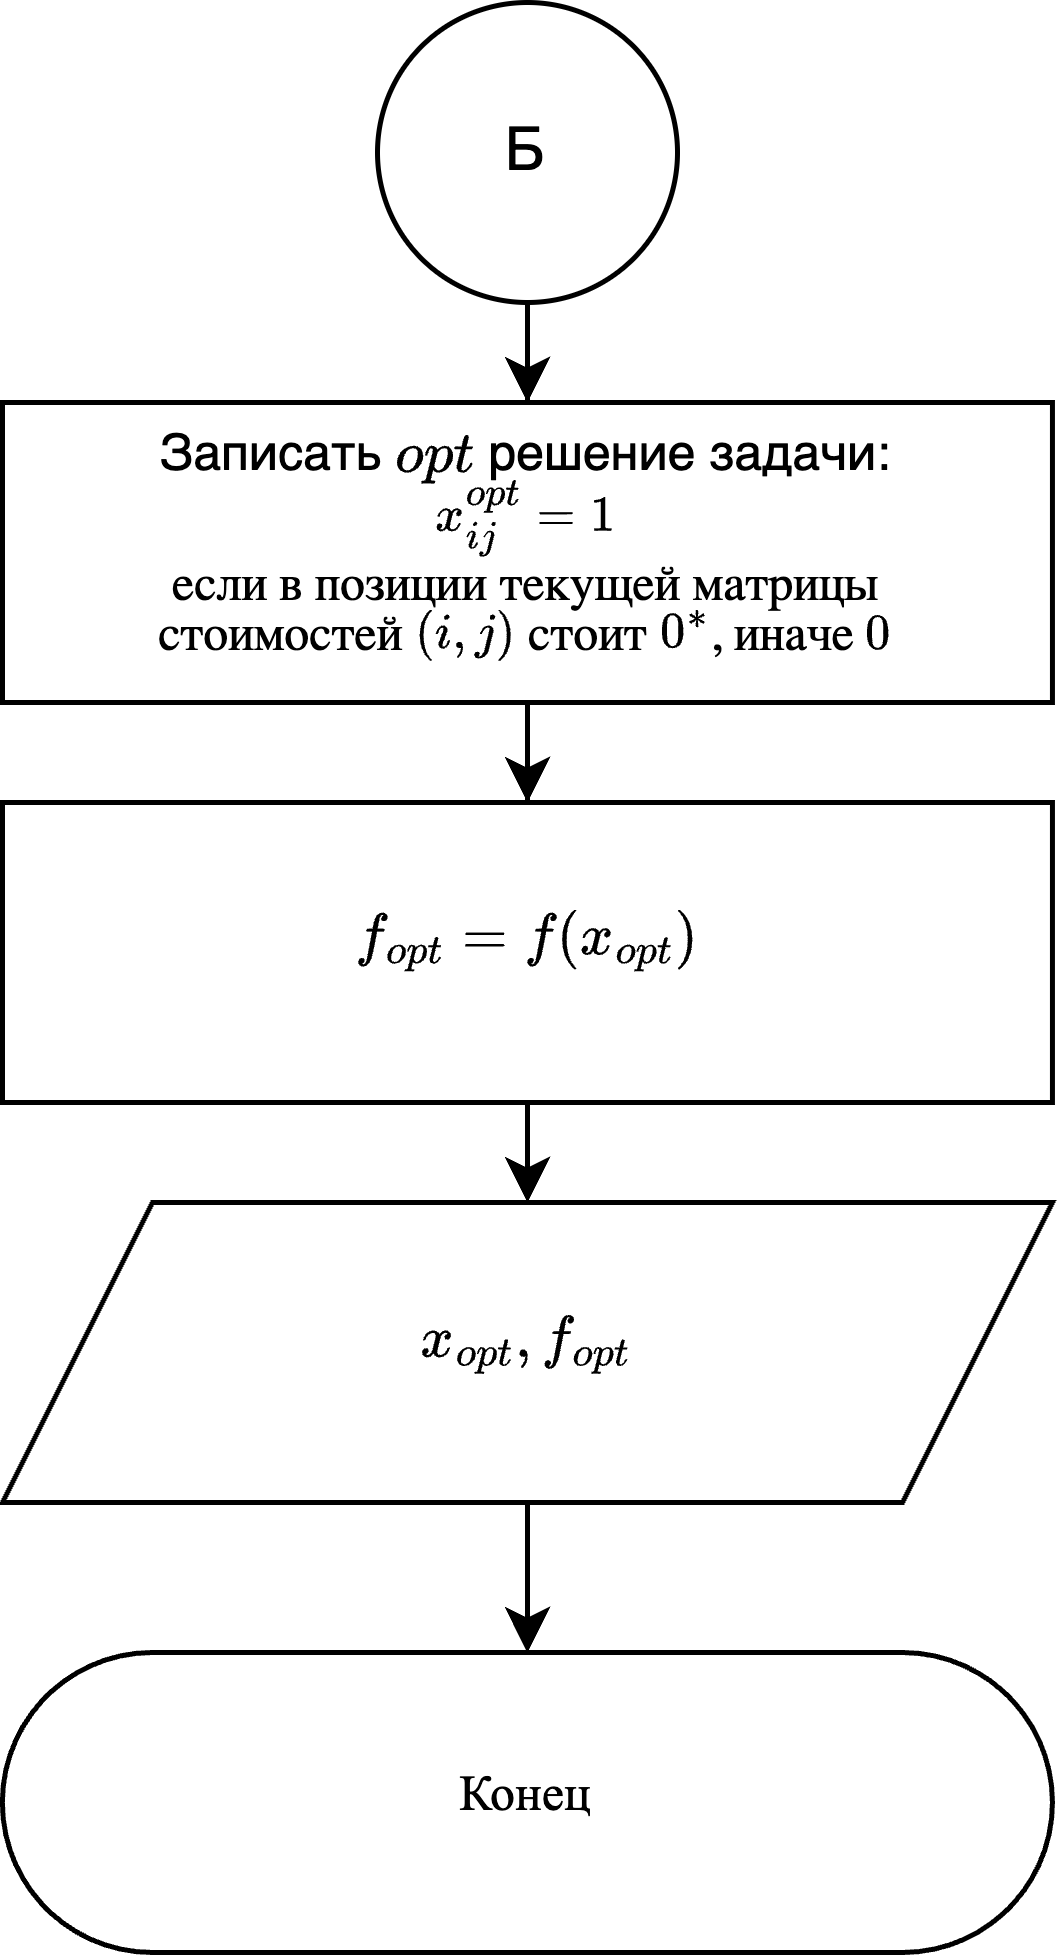
\includegraphics[scale=0.2]{inc/img/3.png}
	\end{center}
	\caption{Схема венгерского метода решения задачи о назначениях, часть 1}
	\label{img:3}
\end{figure}

\chapter{Практическая часть}

\section{Текст программы}

\includelisting{hungarian.m}{Исходный код программы.}

\section{Результаты расчётов для задач из варианта №9}

\includelisting{min-res.txt}{Решение задачи минимизации}

\includelisting{max-res.txt}{Решение задачи максимизации}
	
\end{document}